%!TEX root = ../dissertation.tex

\chapter{Practical Experiments}
\label{chapter:experiments}

The previous sections presented an evaluation based on the development of GD programs and extension of the programming environment. This section completes this evaluation with practical experiments, namely, a comparison of TPLs and VPLs, and conversion and analysis of AutoLISP programs.
Rosetta is a direct descendant of VisualScheme, maintaining the same pedagogical concerns, but with
a different approach: Racket, formerly called Scheme, is still used for the general audience of designers
that do not have a background in Computer Science. However, additional PLs are included and multiple
CAD applications are provided. An additional advantage is the automatic compatibility of the chosen
language with the programming environment and the portability of the programs written in it.
Leitão et al. (Leitão et al., 2012b) compares TPLs and VPLs using VisualScheme and Grasshopper as
representative of TPLs and VPLs, respectively. This comparison is based on a practical experiment to test
program maintenance and adaptability consisting of two tasks, namely, (1) writing a program to create
cylindrical towers (Figure 7.1); and (2) modifying that program to create conical towers with sinusoidal
variations (Figure 7.2). Despite being one of the most popular GD languages, this comparison identifies
several problems in Grasshopper and clearly shows the advantages of VisualScheme over that PL. Being a
descendant of VisualScheme, Rosetta inherits these advantages.

\section{Program-sketch correlation tool}

\begin{figure}[h]
\centering
\begin{minipage}[t]{.495\textwidth}
  \centering
  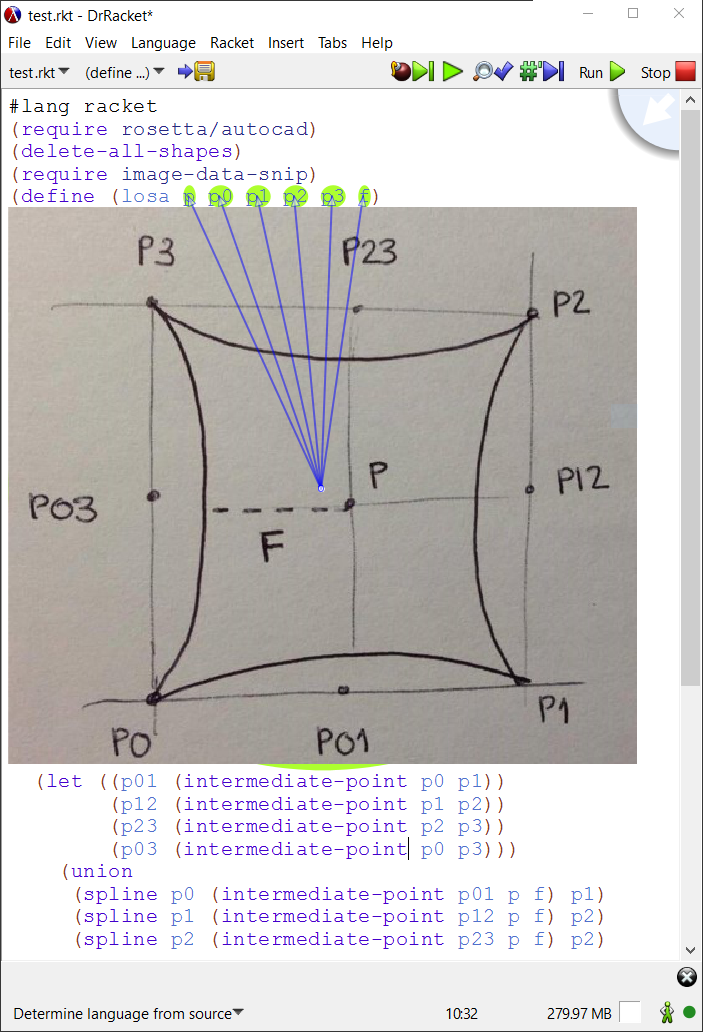
\includegraphics[width=1\linewidth]{images/losa0}
  \captionof{figure}{Relating function arguments with image. The highlighted argument (under the cursor, in green) are illustrated in the image (on the \texttt{R} symbol, using blue arrows).}
  \label{fig:losa0}
\end{minipage}%
~
~
\begin{minipage}[t]{.495\textwidth}
  \centering
  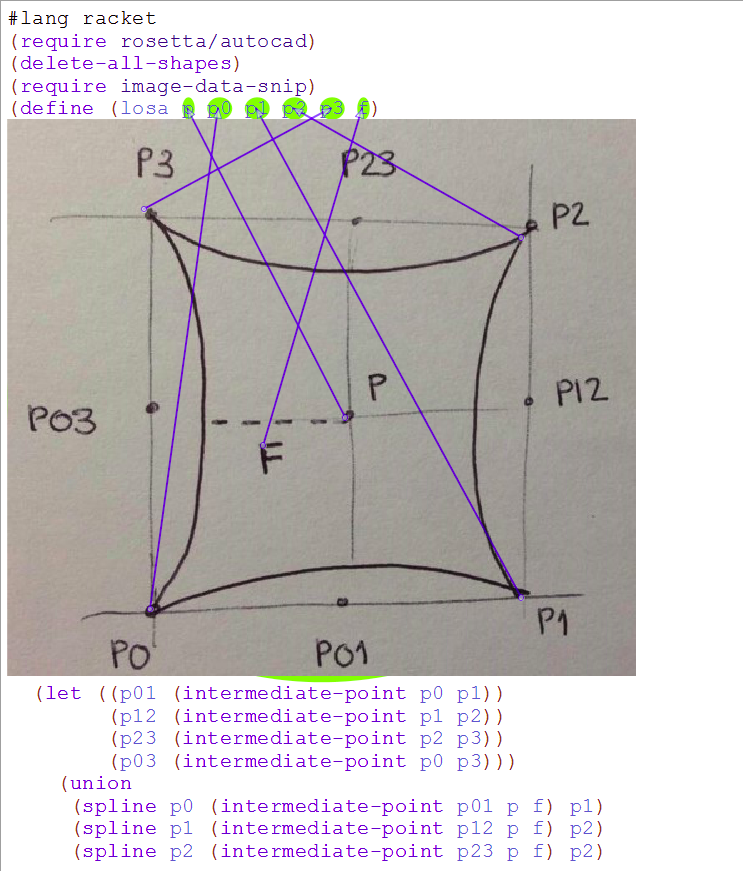
\includegraphics[width=1\linewidth]{images/losa}
  \captionof{figure}{Relating image with function arguments. The parameter illustrated in the image (on the \texttt{c} symbol, under the cursor) are highlighted in the code (in green, using blue arrows).}
  \label{fig:losa1}
\end{minipage}
\end{figure}

\begin{figure}[!h]
  \centering
  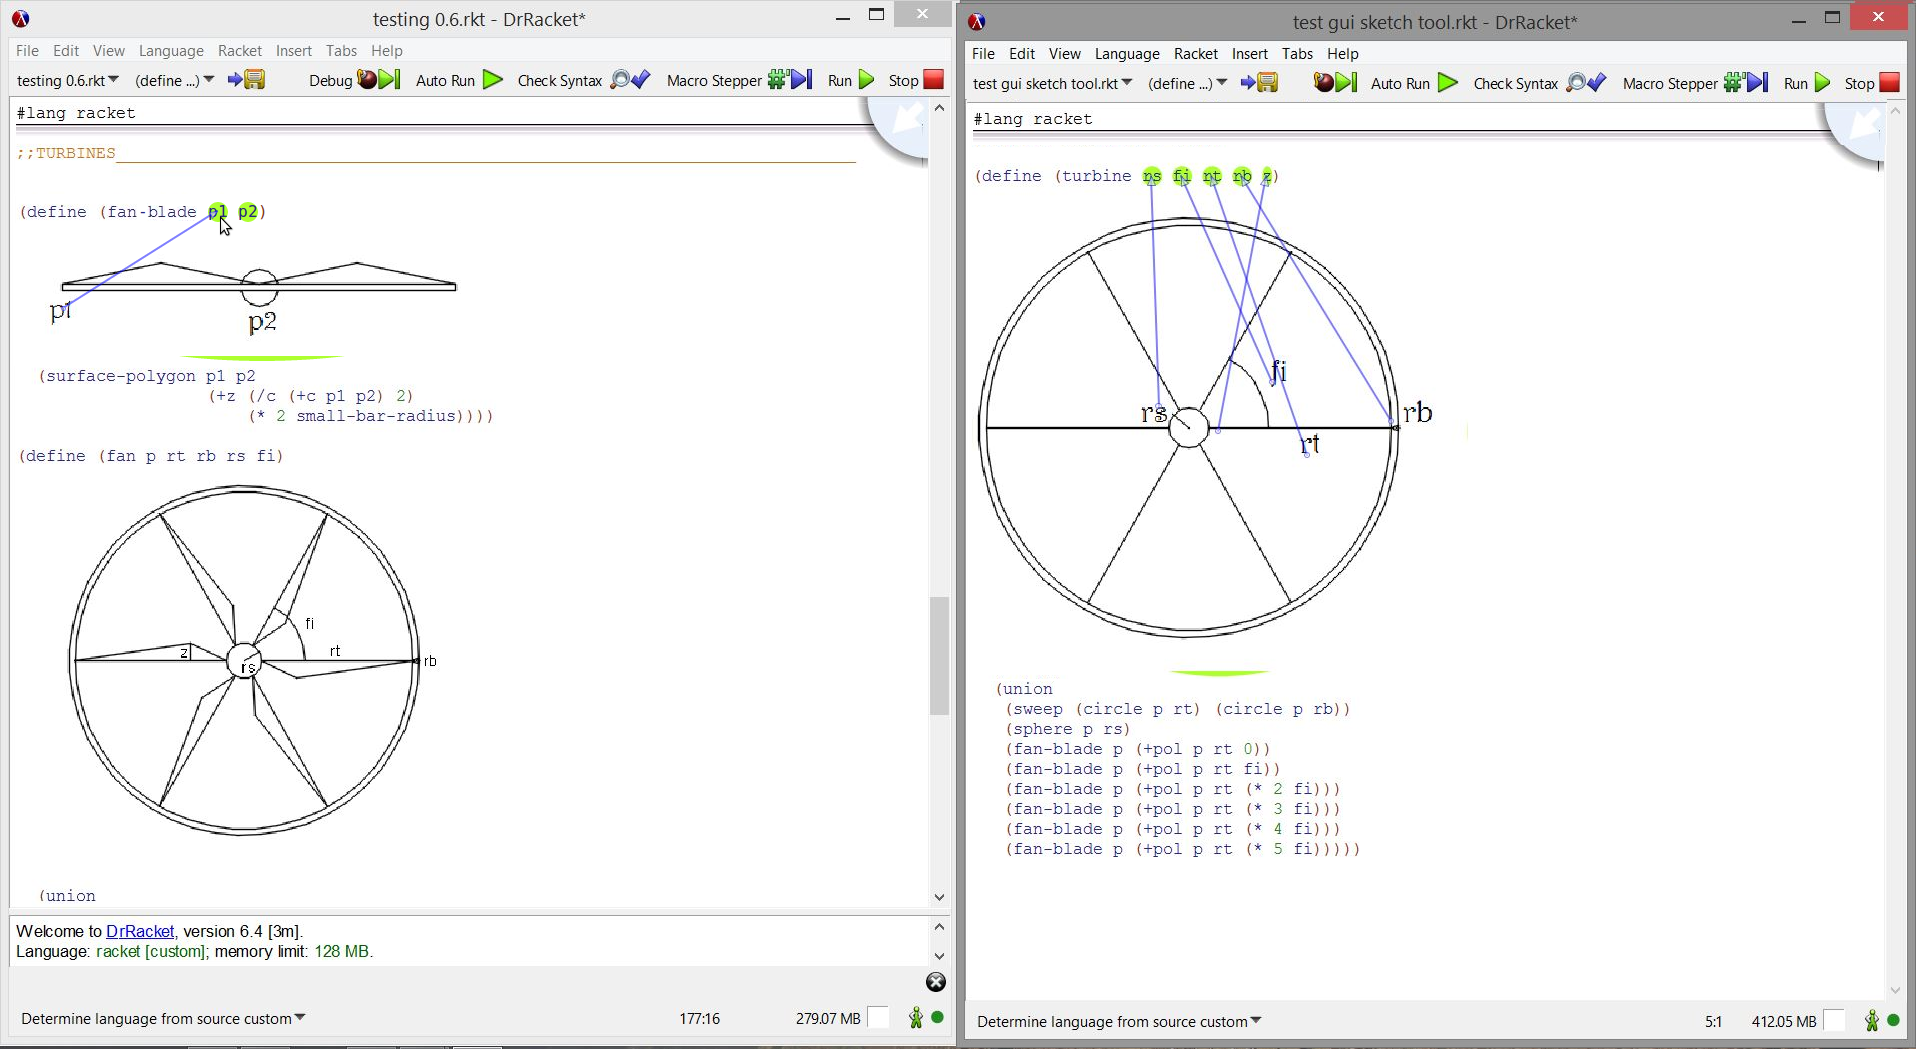
\includegraphics[width=1\textwidth]{images/turbine}
    \caption{Using the slider widget with \textit{Auto Run tool} active, to experiment some input values. The highlighted function call (at line 13, on the left) is being changed by the slider (over the pointer). On the right, are the generated shapes rendered by AutoCAD.}
  \label{fig:turbine}
\end{figure}

\begin{figure}[!h]
  \centering
  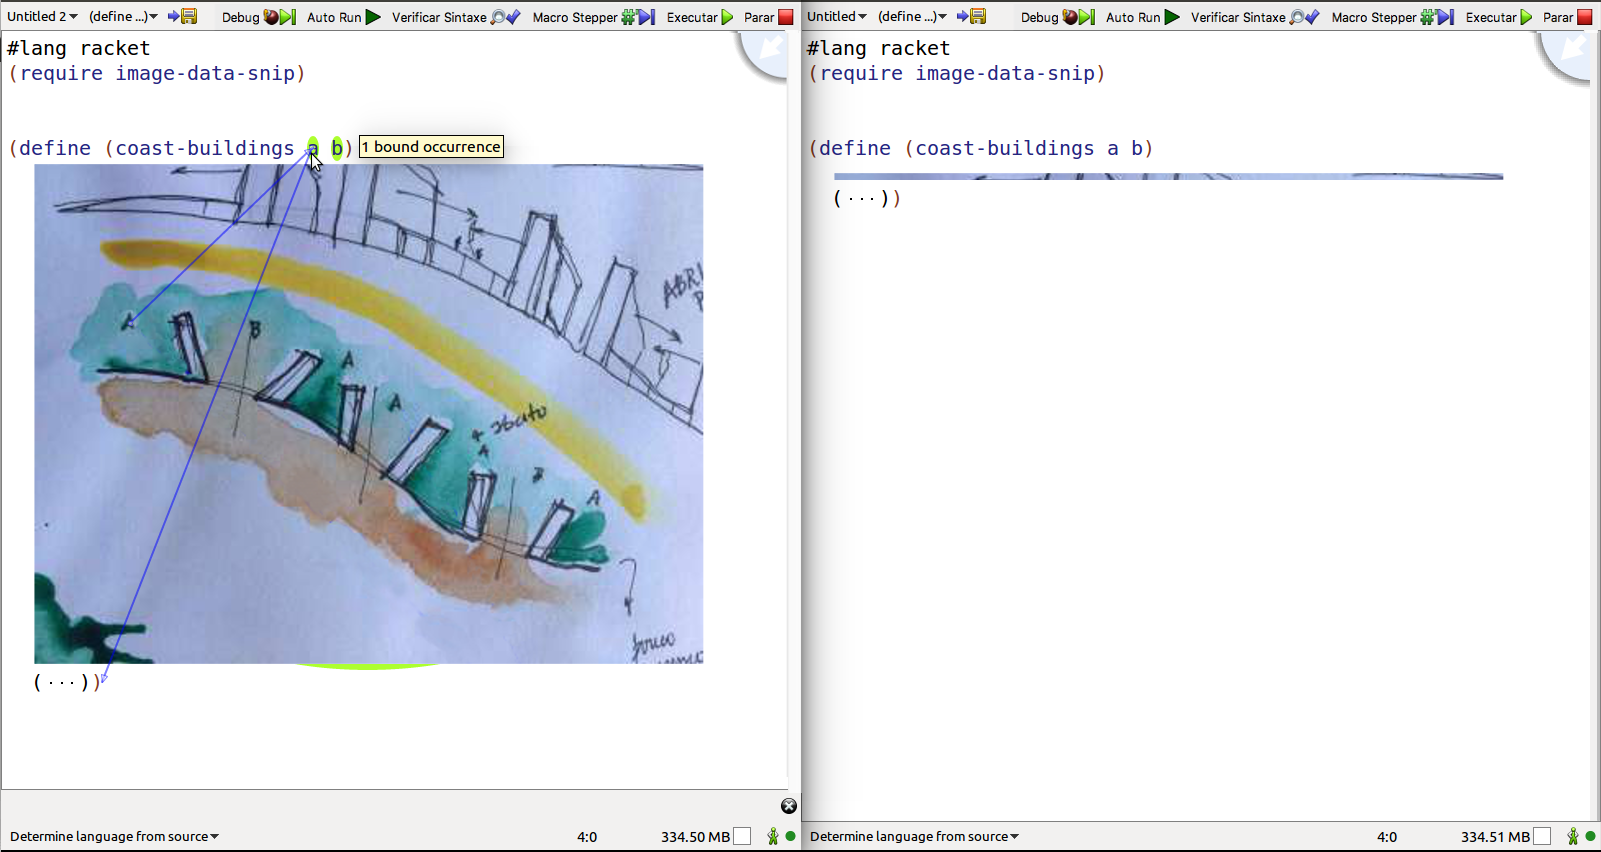
\includegraphics[width=1\textwidth]{images/coast}
    \caption{Using the slider widget with \textit{Auto Run tool} active, to experiment some input values. The highlighted function call (at line 13, on the left) is being changed by the slider (over the pointer). On the right, are the generated shapes rendered by AutoCAD.}
  \label{fig:coast}
\end{figure}


\section{Immediate feedback tool}

\begin{figure}[!h]
  \centering
  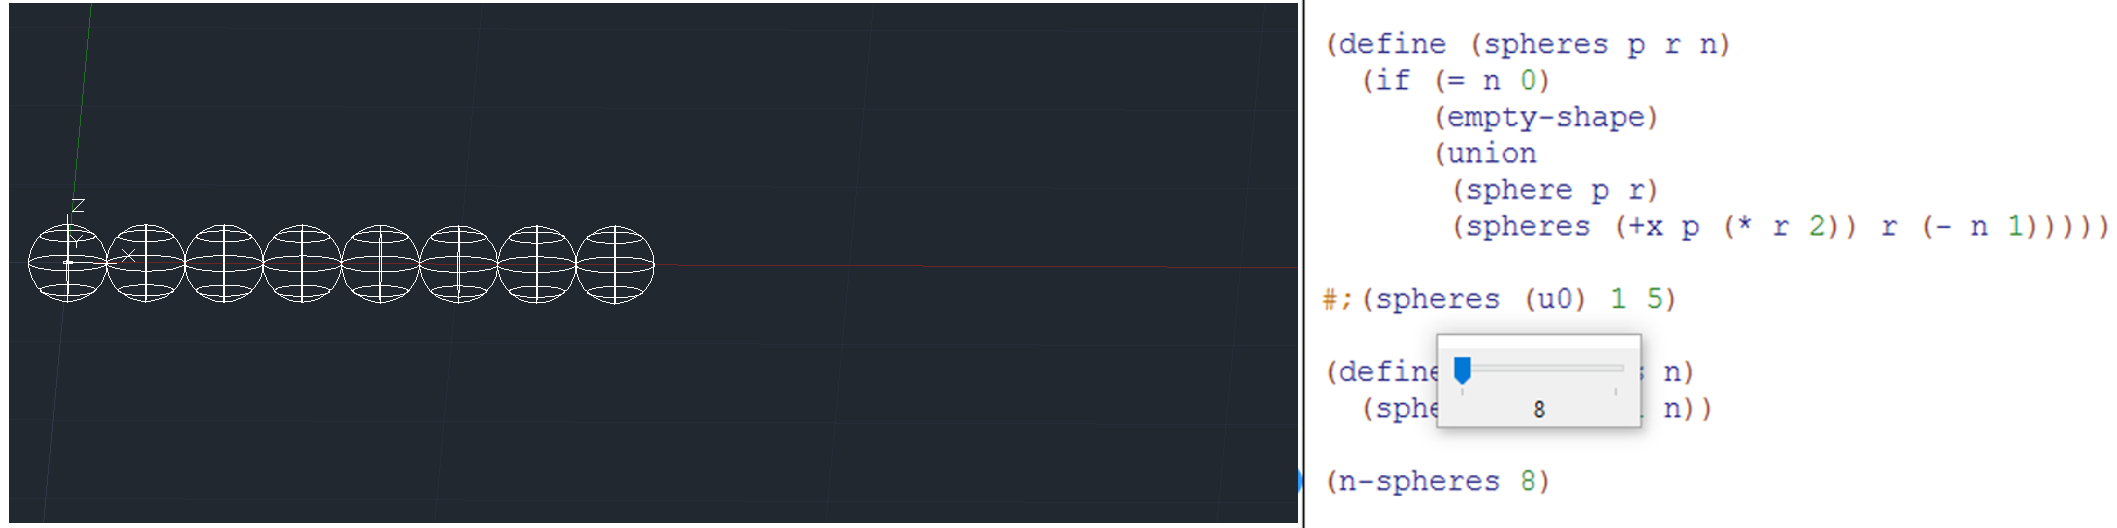
\includegraphics[width=1\textwidth]{images/sliders1}
    \caption{Using the slider widget with \textit{Auto Run tool} active, to experiment some input values. The highlighted function call (at line 13, on the left) is being changed by the slider (over the pointer). On the right, are the generated shapes rendered by AutoCAD.}
  \label{fig:s1}
\end{figure}

\begin{figure}[!h]
  \centering
  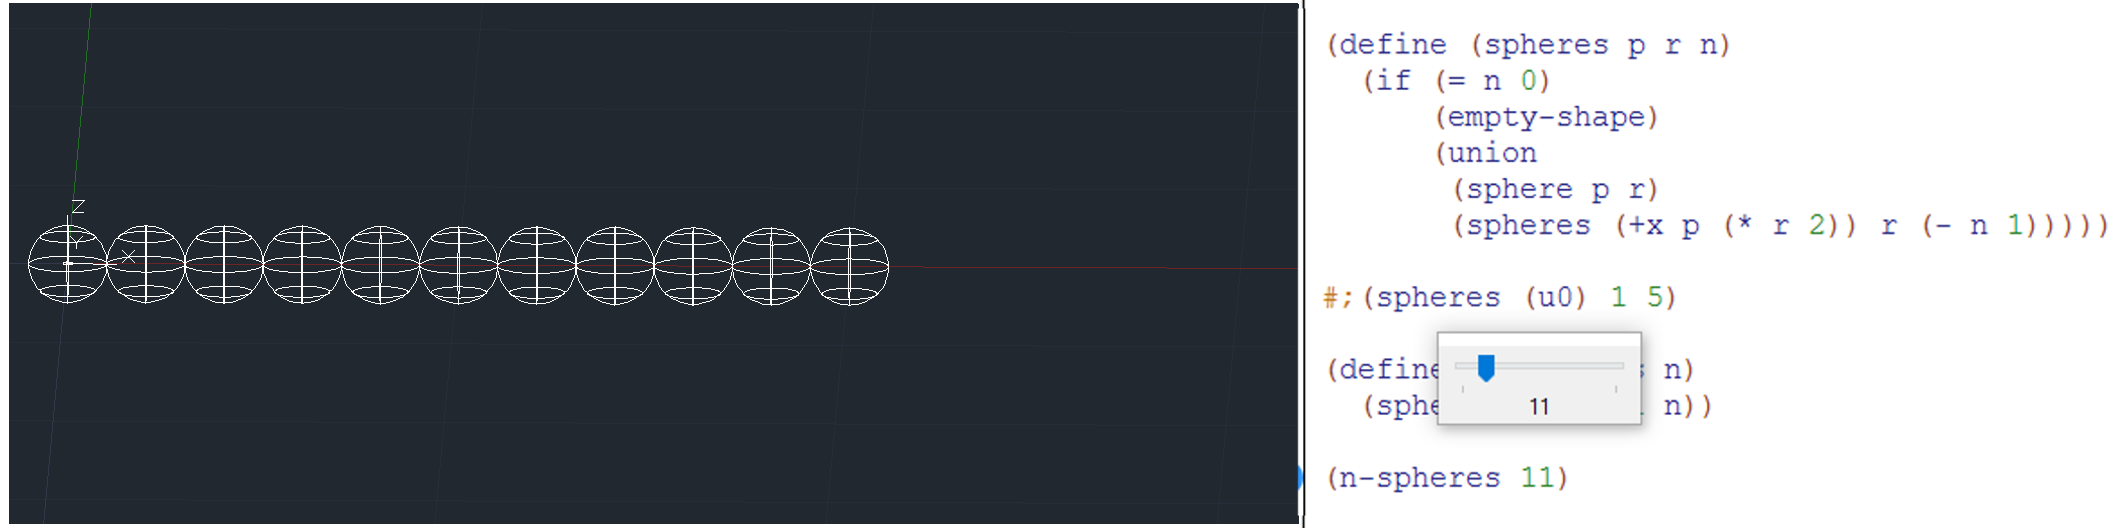
\includegraphics[width=1\textwidth]{images/sliders2}
    \caption{Using the slider widget with \textit{Auto Run tool} active, to experiment some input values. The highlighted function call (at line 13, on the left) is being changed by the slider (over the pointer). On the right, are the generated shapes rendered by AutoCAD.}
  \label{fig:s2}
\end{figure}

\begin{figure}[!h]
  \centering
  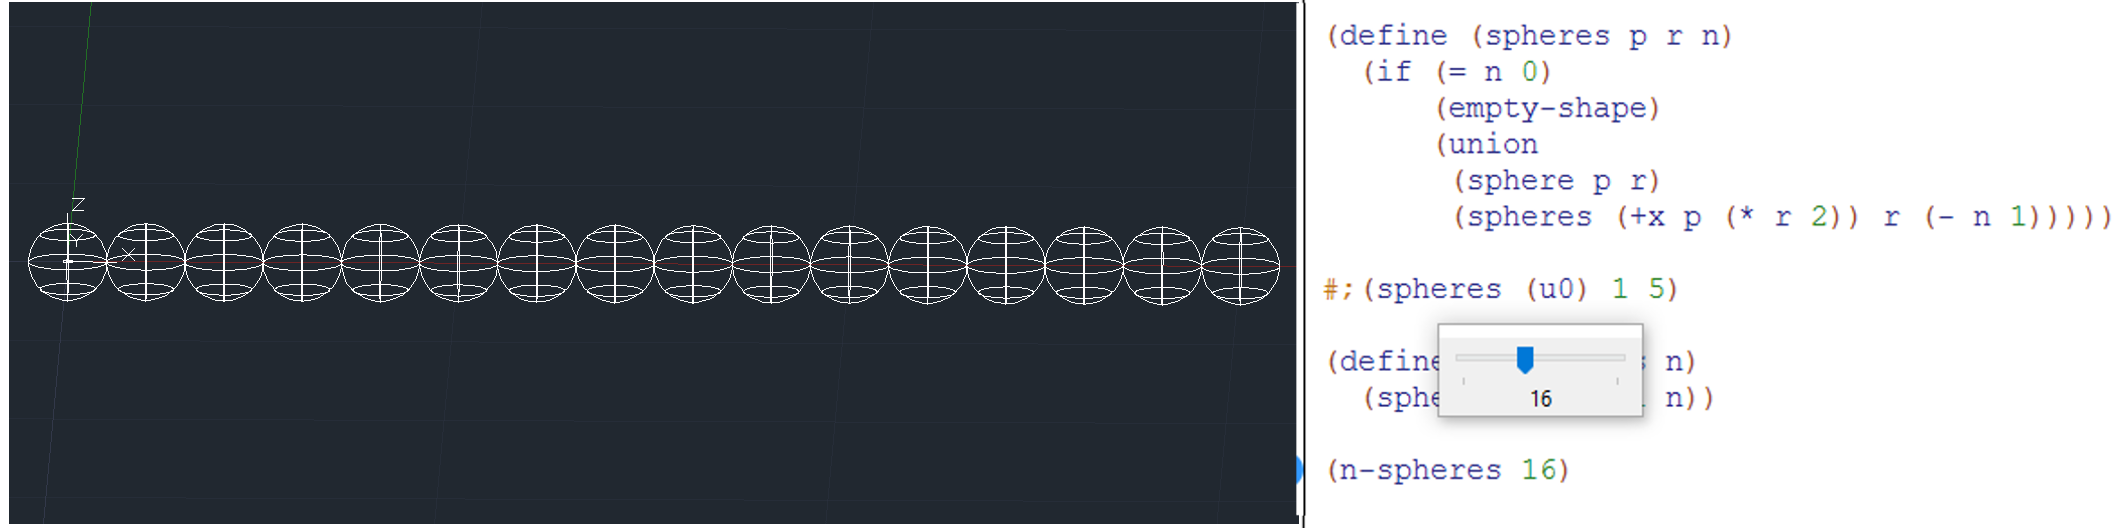
\includegraphics[width=1\textwidth]{images/sliders3}
    \caption{Using the slider widget with \textit{Auto Run tool} active, to experiment some input values. The highlighted function call (at line 13, on the left) is being changed by the slider (over the pointer). On the right, are the generated shapes rendered by AutoCAD.}
  \label{fig:s3}
\end{figure}

\begin{figure}[!h]
  \centering
  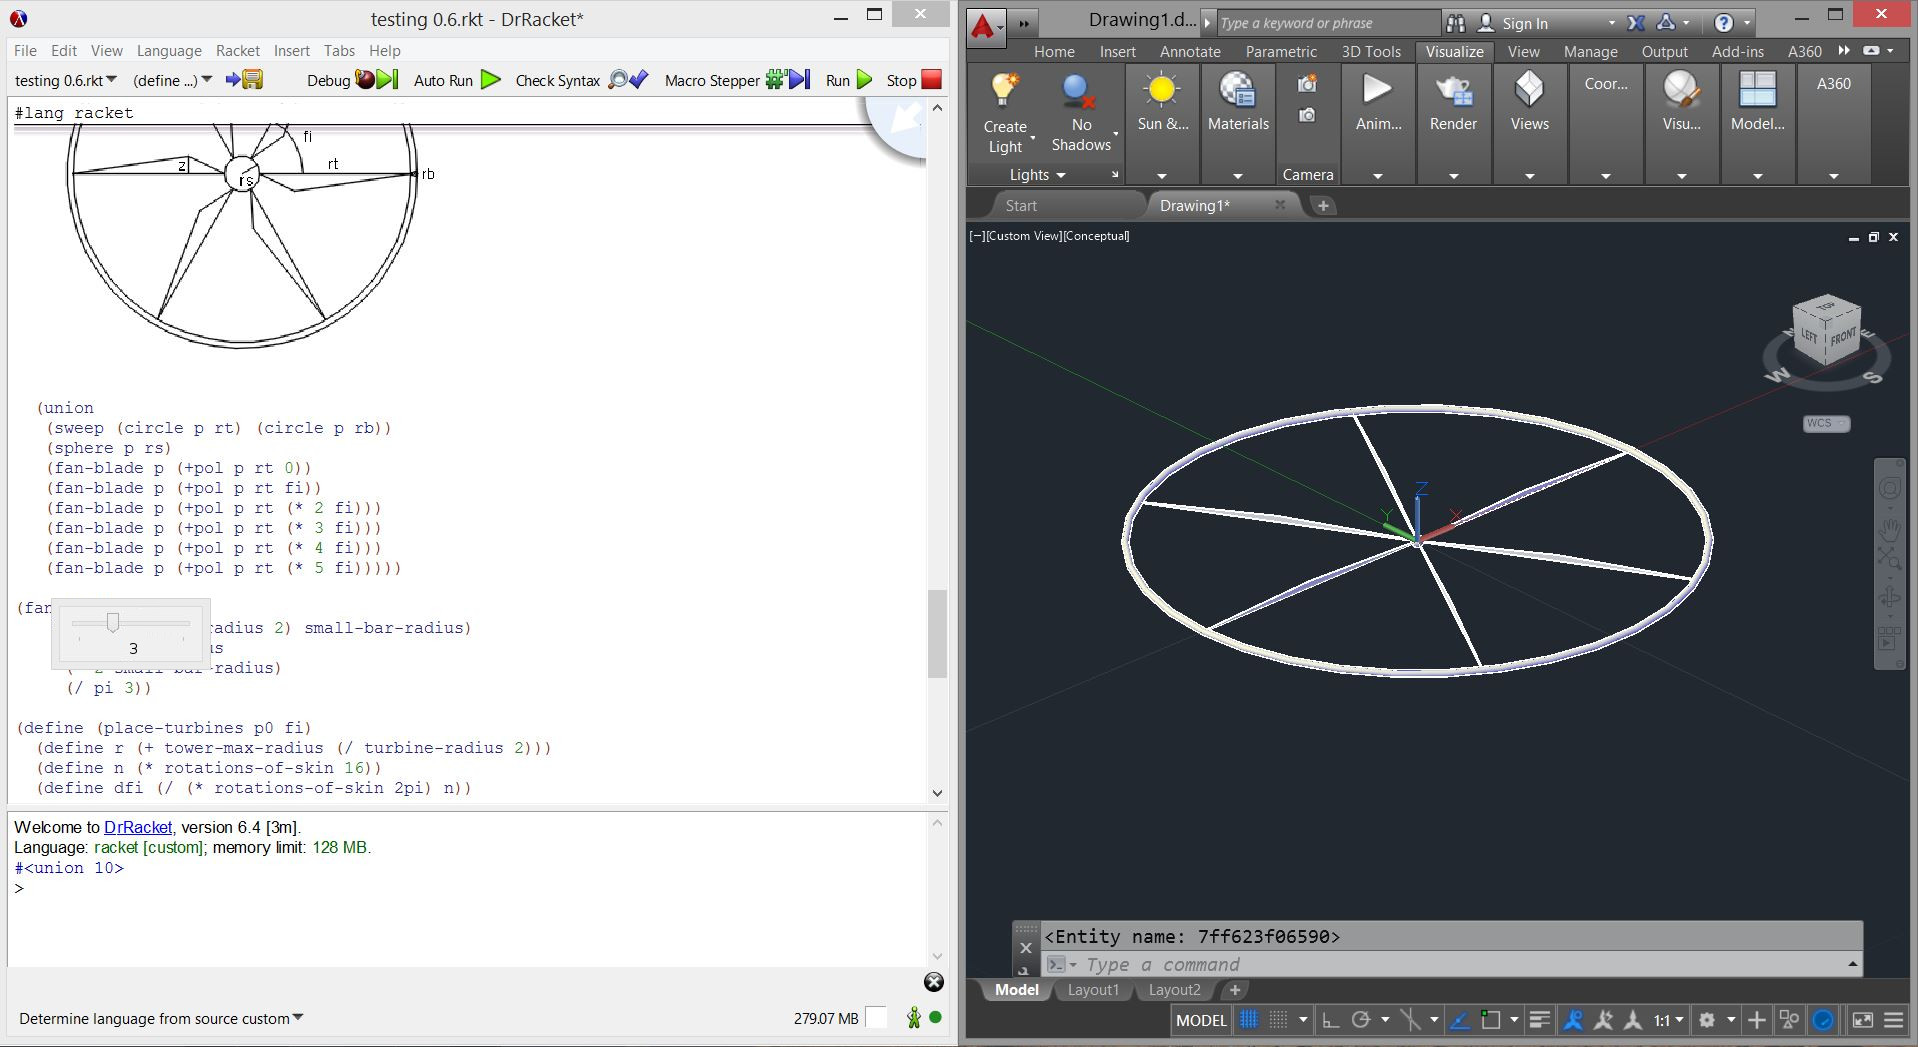
\includegraphics[width=1\textwidth]{images/slider-turbine-1}
    \caption{Using the slider widget with \textit{Auto Run tool} active, to experiment some input values. The highlighted function call (at line 13, on the left) is being changed by the slider (over the pointer). On the right, are the generated shapes rendered by AutoCAD.}
  \label{fig:sturbine1}
\end{figure}

\begin{figure}[!h]
  \centering
  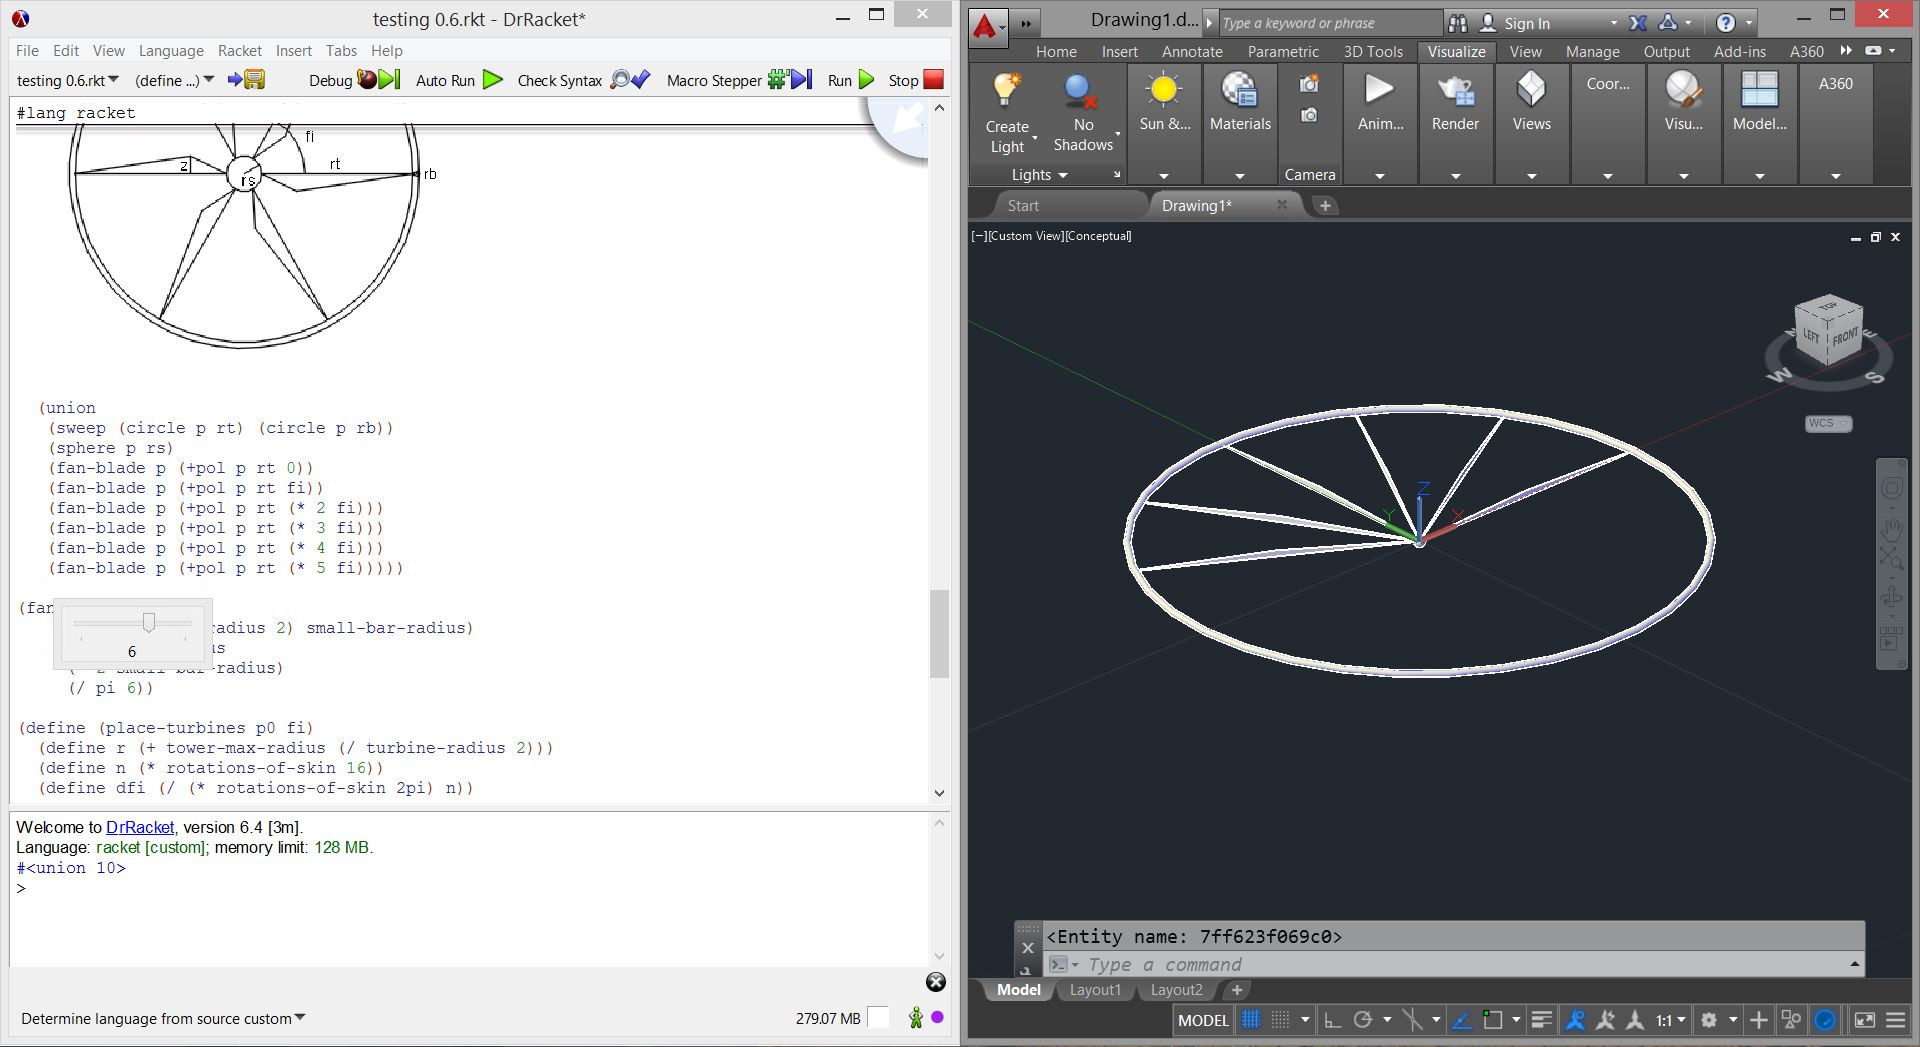
\includegraphics[width=1\textwidth]{images/slider-turbine-2}
    \caption{Using the slider widget with \textit{Auto Run tool} active, to experiment some input values. The highlighted function call (at line 13, on the left) is being changed by the slider (over the pointer). On the right, are the generated shapes rendered by AutoCAD.}
  \label{fig:sturbine2}
\end{figure}

\begin{figure}[!h]
  \centering
  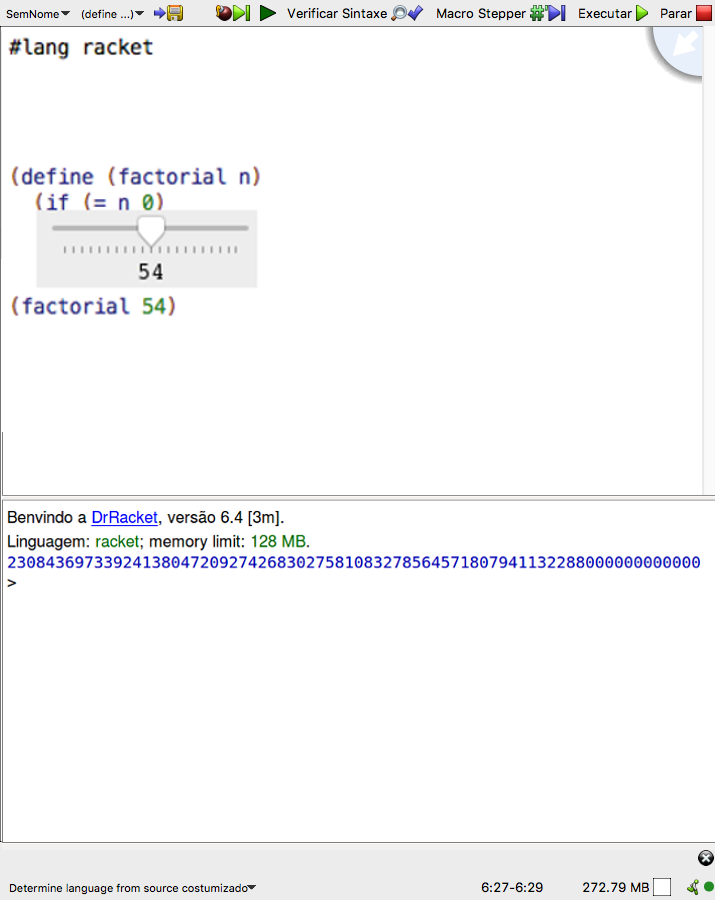
\includegraphics[width=0.5\textwidth]{images/slider-mac}
    \caption{Using the slider widget with \textit{Auto Run tool} active, to experiment some input values. The highlighted function call (at line 13, on the left) is being changed by the slider (over the pointer). On the right, are the generated shapes rendered by AutoCAD.}
  \label{fig:slidermac}
\end{figure}


\section{Evaluation}
\label{sec:eval}

The evaluation of the proposed architecture will be performed experimentally, building a prototype. The prototype will serve to test the proposed ideas and to evaluate them. To evaluate the prototype, we will use the Rosetta~\citep{lopes2011portable} generative design tool as a case study. As Rosetta is used by architects, and designer, we will receive real feedback from the target users. In this way, we can evaluate if our programming environment helps their target users to design programs.

Furthermore, to evaluate our proposal we plan to use the following evaluation metrics.

\begin{itemize}
\item \textbf{Correctness.} To assess the quality of our system we plan to test, individually, each proposed feature with a specific test case scenario, for example using the slider widget to explore the result of a parametric function and inserting different kinds of images and check if the image is well correlated with the function parameters. 

\item \textbf{Security.} Among others qualities, security is an important concern in a live environment where the code is executed instantly. In our case, the code is executed locally, however while the users are using the live code mode they can create dangerous constructs such as \texttt{eval}, \texttt{exec} and \texttt{file I/O} which can damage the operating system. On the other hand, in this mode it is possible to block the environment with a simple ``while true'' expression. To avoid these problems, we plan to implement sandboxing, similar to PythonTutor~\citep{GuoSIGCSE2013}, and design specific tests to test this feature.

\item \textbf{Performance.} The performance of our system should scale for the generative design programs. The Rosetta tool will give us different \textit{backends} to test the performance of our interactive tool. In fact, to be an interactive tool, the response for an event should be quick ($\sim$50ms). It imposes restrict requirements for the CADs tools, because these tools were designed for the speed of human operation, consequently they are the performance bottleneck. This issue forces us to establish a limit which this tool will be tested, thus we will compare this limit against other similar systems.

\item \textbf{Comparison with other systems.} We can only claim that our solution is somehow better than the other, if we compare them. Therefore, we plan to compare our system with the existing programming environments in generative design, particularly the visual environments, such as Grasshopper. Between these systems, the performance limit, stated above, will be our reference of comparison.
\end{itemize}



- note-se que as imagens deveriam ter algumas dimensoes
  antes de serem colocadas no editor.
  
-example of architect sketches
 um ou dois paragrafos a descrever
 com a imagem 

-util immediate feecback

-criticas
 mais vaga, dificuldades no tamanho da imagem
 ferramentas externas que podem ajustar a imagem
 
 feedback imediato, nos backends preferidos pelos
 arquitectos pode nao ser tao imediato.

 slider adaptativo..
